\chapter{Atividade Econômica}
\par A eclosão da pandemia do coronavírus tem se mostrado o maior choque enfrentado pela economia brasileira, tanto pela demanda com a contração do consumo das famílias e dos investimentos, quanto pelo lado da oferta, com empresas indo à falência. Compondo a isso se tem a fragilidade fiscal do Estado brasileiro e a alta taxa de desemprego desde a recessão de 2015/2016. Dado este contexto, cria-se cenário preocupante para a economia brasileira como um todo.
\par Nesse sentido, espera-se também um grande choque na economia tocantinense. Os indicadores que serão apresentados ao longo das seções deste Boletim farão um retrato de como esse grande choque afetou e poderá afetar a economia do nosso estado.
\begin{figure}[!h]
	\begin{subfigure}{\linewidth}
		\caption{Expectativa de crescimento anual do PIB}
		\subcap{Mediana por setor}
		\label{fig:expectativa_pib}
		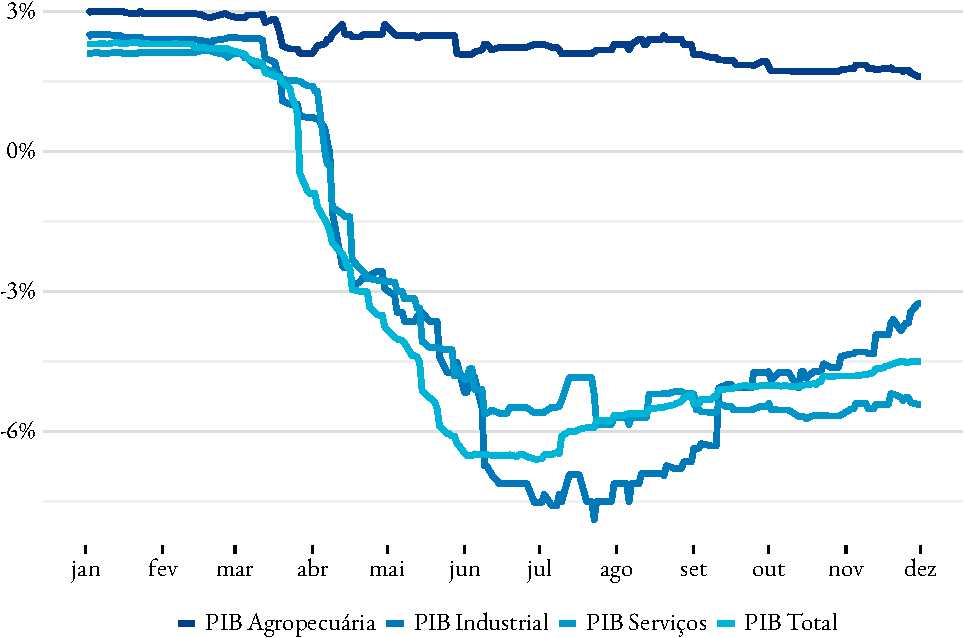
\includegraphics{fig/pib_expec-1.pdf}
		\source{\acrshort{bcb}}
	\end{subfigure}
	\begin{subfigure}{\linewidth}
		\caption{Variação trimestral do PIB pelo lado da demanda}
		\subcap{Com ajuste sazonal}
		\label{fig:pib_demanda}
		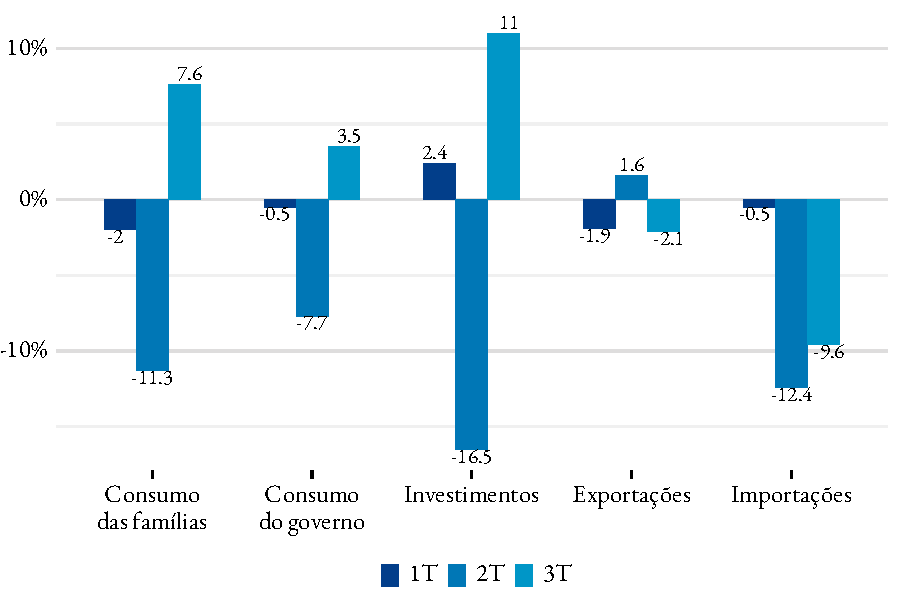
\includegraphics{fig/pib_demanda.pdf}
		\source{\acrshort{ibge}}
		\notes{1T: 1º trimestre, 2T: 2º trimestre, 3T: 3º trimestre}
	\end{subfigure}
	\begin{subfigure}{\linewidth}
		\caption{Variação trimestral do PIB pelo lado da oferta}
		\subcap{Com ajuste sazonal}
		\label{fig:pib_oferta}
		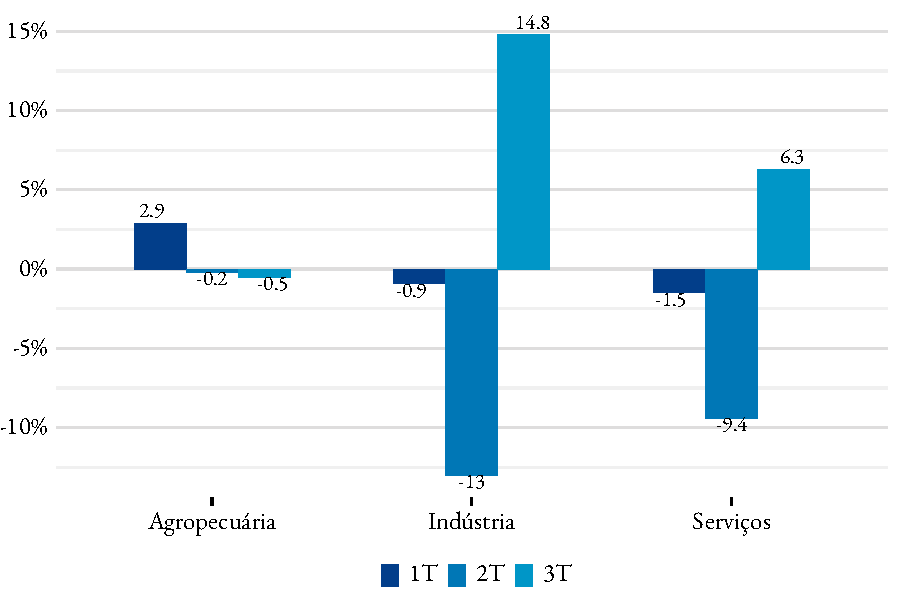
\includegraphics{fig/pib_oferta.pdf}
		\source{\acrshort{ibge}}
		\notes{1T: 1º trimestre, 2T: 2º trimestre, 3T: 3º trimestre}
	\end{subfigure}
\end{figure}
\par No início do ano a mediana das expectativas de crescimento para a economia brasilera situava-se em torno de 2,3\%, indústria e serviços seguiam com expectativa de crescimento próxima, agropecuária um pouco deslocada com uma expectatvia acima do PIB agregado, 2,95\% -- figura \ref{fig:expectativa_pib}. Até o final do primeiro trimestre as expectativas se mantiveram nesse nível, apresentando pouca variação. No primeiro trimestre a economia encolheu 1.5\% com a maior contração no consumo das famílias e nas exportações, -2\% e -1,9\% respectivamente. Investimento foi o único que apresentou um crescimento de 2,4\%.
\par A partir do meio março as expectativas começam a reduzir, ao final de março as projeções apontavam contração em todos os setores, exceto o agropecuário com expectativa acima de 1,5\%.
\par No acumulado nos três primeiros trimestres de 2020 o PIB brasileiro encolheu 1,5\% e 9,6\%, nos dois primeiros trimestres teve um crescimento de 7,7\% no terceiro, que apesar de alto, ainda não foi suficiente para repor as perdas no início do ano. Esses resultados foram os primeiros sinais dos efeitos da pandemia da COVID-19, sendo que seu resultado negativo em partes explicados pelas medidas de fechamento de comércios e serviços a fim de evitar a propagação do vírus, sobretudo no segundo semestre.
\par No lado da demanda na figura \ref{fig:pib_demanda} é possível ver uma queda generalizada sobre todos os componentes, com exceção das exportações. Chama a atenção as fortes quedas no segundo trimestre, sobretudo no consumo das famílias, investimentos e importações. No movimento de retomada do terceiro semestre é possível observar que grande parte do aumento de 7,7\% é explicado pela retomada do Consumo das famílias e Investimentos, tanto pelos bons resultados neste trimestre, mas também pelo tamanho desses componentes dentro da composição do PIB.
\par Pelo lado da oferta apresentado na figura \ref{fig:pib_oferta} o único setor com resultados mais estáveis foi o Agropecuário, setor menos afetado pelas medidas de isolamento, e o que em parte explica o bom desempenho das exportações no lado da demanda. No setor de serviços, que representa mais que 70\% do PIB, as quedas de 1.5\% e 9,4\% nos dois primeiros trimestres pesaram bastante. Já as quedas de 0,9\% e 13\% da indústria demonstram a fragilidade desse setor dentro da economia brasileira.
\par No quarto trimestre as expectativas do PIB total apresentou um leve crescimento, as últimas projeções de 2020 apontam contração de -4,36\%. Já a mediana das expectativas do PIB da industria mostrou uma leve recuperação nos útimos três meses, finalizando o ano com -3,9\%. Serviçõs também exibiu uma tímida recuperação, finalizando com -4,8\%. O setor agropecuário, menos afetado, ao longo de todo o ano teve expectativa de crescimento acima de 1,5\%, teve reduções ao longo de 2020, mas finalizou o ano com projeção de crescimento de 2,32\%.

\begin{smbox}[label={labelbox},nameref={Cálculo do PIB e as suas óticas}]{Cálculo do PIB e as suas óticas}
	O Produto Interno Bruto (\acrshort{pib}) é a soma de todos os bens e serviços finais produzidos por um país. É possível calcula-lo por três óticas diferenets, pela oferta, somando tudo aquilo que é produzido por todos os setores, pela da demanda, somando o consumo das famílias, consumo do governo, investimentos e exportações liquidas (exportações menos importações) e também pela ótica da renda, somando toda renda da população. O resultado das três óticas é sempre o mesmo.
\end{smbox}


\par Um outro ponto a ser analisado no contexto de atividade econômica é a Pesquisa Mensal do Comércio (\acrshort{pmc}). Nela são demonstrados informações para a análise e compreensão do comércio. A função clara do PMC é transpor índices dos comércios para a sociedade e por consequência, relatarem o movimento do setor no período.

 \begin{smbox}[label={labelbox},nameref={Pesquisa Mensal do Comércio(PMC)}]{Pesquisa Mensal do Comércio (PMC)}
	A pesquisa é realizada desde dos anos 80, pelo IBGE, é divulgada mensalmente e para todos os estados da federação. Essas variações são compostas por inúmeras atividades como comércio varejista, combustíveis e lubrificantes, hipermercados, supermercados, produtos alimentícios, bebidas e fumo, tecidos, vestuário e calçados, móveis e eletrodomésticos, artigos farmacêuticos, médicos, ortopédicos, de perfumaria e cosméticos, livros, jornais, revistas e papelaria, equipamentos e materiais para escritório, informática e comunicação, outros artigos de uso pessoal e doméstico.
 \end{smbox}

\par A atividade comercial no estado do Tocantins é de grande importância para a construção do PIB estadual. Até a atual formulação deste boletim, são apresentados dois índices que compõe a PMC, são eles: Serviços e Vendas no comércio varejista.
\par Na Figura \ref{fig:pmc}, o setor de serviços sofrem com maiores variações. Analisando os dados a partir de março de 2019 até setembro do nosso ano de exercício, é apresentado uma recuperação desse setor até Março do ano atual. Uma justificativa para as variações negativas do setor de serviços até o atual momento, são as medidas de isolamento social para a contenção do Covid-19, assim, se encerra um período de variações positivas no setor que teve inicio em março de 2019.
\par O comércio varejista tem uma relação evidente com o setor de serviços, entretanto, não sofreu com altas variações como o setor de serviços. Em março de 2019, o setor vinha de uma queda semelhante ao de serviços, mas, a partir desse momento obteve variações positivas até março do atual ano. A queda na variação do comércio varejista foi amenizada, mesmo no contexto da Covid-19 pelos estímulos que a economia recebeu para lidar com a atual pandemia, o que pode se justificar essa queda mais suavizada do que o setor de serviços.
\begin{figure}[!h]
	\begin{subfigure}{\linewidth}
		\caption{Atividade Econômica do Estado}
		\label{fig:pmc}
		\subcap{Variação acumulada no ano (base: igual período do ano anterior)}
		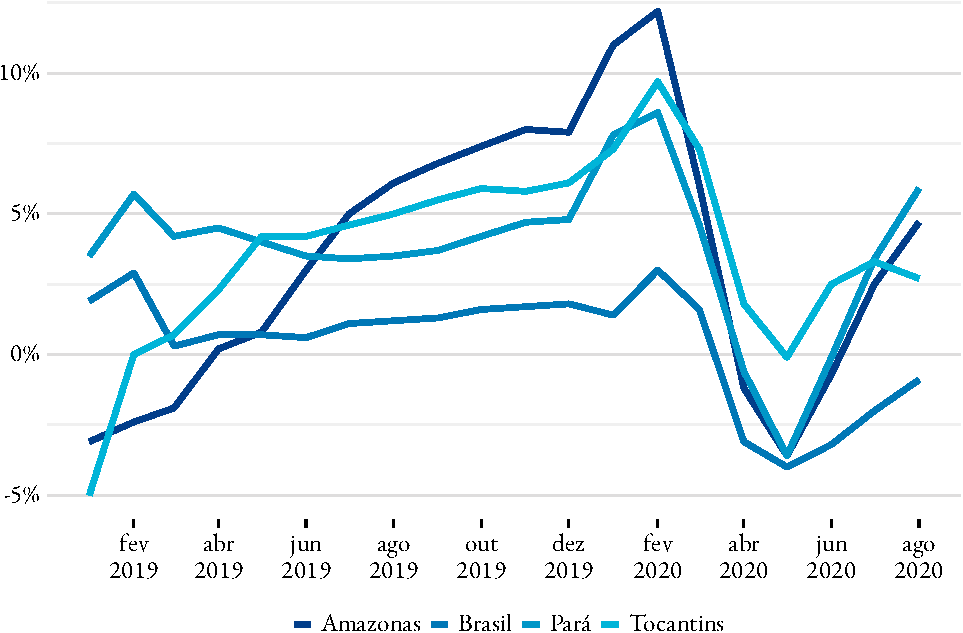
\includegraphics{fig/pmc_ibge-1.pdf}
		\source{IBGE}
	\end{subfigure}
\end{figure}

